% ============================================================
%  HCMIU Map Collaborative — Beamer Presentation
%  Course : Advanced Database System (IT502IU)
%  Student: Huynh Tran Khanh (MITIU25210)
%  Duration: ~8 minutes
% ============================================================
\documentclass[aspectratio=169,11pt]{beamer}

% ---------- Theme & colours ----------
\usetheme{Madrid}
\usecolortheme{seahorse}
\setbeamertemplate{navigation symbols}{}
\setbeamertemplate{footline}[frame number]

% ---------- Packages ----------
\usepackage[T1]{fontenc}
\usepackage[utf8]{inputenc}
\usepackage{graphicx}
\usepackage{booktabs}
\usepackage{hyperref}
\usepackage{tikz}
\usepackage{listings}
\usepackage{xcolor}
\usepackage{pgfpages}

% ---------- Presenter notes ----------
% Uncomment the next line to show notes on a second screen:
% \setbeameroption{show notes on second screen=right}
% For a printable version with notes below each slide:
\setbeameroption{show notes}
\setbeamertemplate{note page}{%
  \vskip1em
  \begin{minipage}[t]{0.95\textwidth}
    \scriptsize
    \insertnote
  \end{minipage}
}

% ---------- Graphics path ----------
\graphicspath{{../docs/screenshots/}}

% ---------- Listings style ----------
\lstset{
  basicstyle=\ttfamily\scriptsize,
  breaklines=true,
  frame=single,
  backgroundcolor=\color{gray!10},
  keywordstyle=\color{blue!70!black},
  commentstyle=\color{green!50!black},
  showstringspaces=false
}

% ---------- Metadata ----------
\title[HCMIU Map Collaborative]{%
  HCMIU Map Collaborative\\[4pt]
  \small A Multi-Model Database-Driven Campus Map\\
  with Real-Time Collaboration}
\author{Huynh Tran Khanh \\ \small Student ID: MITIU25210}
\institute{%
  Advanced Database System (IT502IU)\\
  International University --- VNU-HCM}
\date{\today}

% ============================================================
\begin{document}

% --------------------------------------------------
% SLIDE 1: Title
% --------------------------------------------------
\begin{frame}
  \titlepage
\note{
Good morning/afternoon. My name is Huynh Tran Khanh.
Today I will present my individual DBMS application project:
HCMIU Map Collaborative---a web-based campus map platform
that combines indoor navigation with a collaborative knowledge graph,
all powered by ArangoDB's multi-model architecture.
The presentation will cover the motivation, system design,
key features, database design, a live demonstration, and conclusions.
}
\end{frame}

% --------------------------------------------------
% SLIDE 2: Outline
% --------------------------------------------------
\begin{frame}{Outline}
  \tableofcontents
\note{
Here is the roadmap for the next eight minutes.
We start with motivation and problem context,
then move into system architecture and the database model.
After that I will walk through the four main feature groups:
campus navigation, collaborative knowledge graph, the trial system,
and the research toolkit.
We will look at screenshots of the running system,
discuss the technology stack, and wrap up with conclusions and future work.
}
\end{frame}

% ============================================================
\section{Introduction \& Motivation}
% ============================================================

% --------------------------------------------------
% SLIDE 3: Problem Context
% --------------------------------------------------
\begin{frame}{Problem Context}
  \begin{columns}[T]
    \begin{column}{0.55\textwidth}
      \textbf{Challenge:} Campus information systems must handle
      \begin{itemize}
        \item \textbf{High schema variability} --- rooms, notes, comments,
              trials, moderation records evolve over time
        \item \textbf{High relationship density} --- references, follows,
              replies, dispute participants form a dense graph
      \end{itemize}
      \vspace{0.5em}
      \textbf{Traditional approach:}
      Polyglot persistence (separate document store + graph DB)
      $\Rightarrow$ operational overhead, synchronisation burden
      \cite{stonebraker2005onesize, sadalage2012nosql}
    \end{column}
    \begin{column}{0.42\textwidth}
      \begin{block}{Our Approach}
        Use \textbf{ArangoDB}---a single multi-model engine that
        natively supports documents, graphs, and key-value
        workloads---to reduce impedance mismatch while keeping
        full graph query power.
      \end{block}
    \end{column}
  \end{columns}
\note{
The core problem is that campus information is both highly variable
in structure---new entity types keep appearing---and highly connected.
Traditional solutions either use a single relational database,
which struggles with graph queries, or polyglot persistence,
which introduces operational complexity.
Our approach is to use ArangoDB, a multi-model DBMS that handles
documents and graphs in one engine, eliminating cross-system coordination.
This is consistent with Stonebraker's argument that one-size-fits-all
is rarely optimal, but here a multi-model engine can cover both needs.
}
\end{frame}

% --------------------------------------------------
% SLIDE 4: Project Objectives
% --------------------------------------------------
\begin{frame}{Project Objectives}
  \begin{enumerate}
    \item \textbf{Interactive campus navigation} ---
          7-floor indoor map with BFS shortest-path and
          Traveling Salesman (Held--Karp) multi-stop optimiser
    \item \textbf{Collaborative knowledge graph} ---
          entity-based discussions with cross-references,
          follows, notifications, and an activity feed
    \item \textbf{Transparent dispute resolution} ---
          a structured ``Court of Justice'' trial system
          with judge negotiation and voting
    \item \textbf{Graph-native research tools} ---
          reference discovery, full-text search,
          degree-of-separation queries
    \item \textbf{Real-time experience} ---
          WebSocket event propagation for live updates
  \end{enumerate}
\note{
These are the five concrete objectives.
First, we build an interactive 7-floor campus map with two pathfinding
algorithms: BFS for point-to-point shortest path, and
the Held-Karp bitmask DP algorithm for the Traveling Salesman Problem.
Second, we create a collaborative knowledge graph where every room,
user, post, and comment is an entity connected by typed edges.
Third, we implement a court trial system for dispute resolution.
Fourth, we provide research tools that exploit the graph model.
And fifth, everything updates in real time via WebSockets.
}
\end{frame}

% ============================================================
\section{System Architecture}
% ============================================================

% --------------------------------------------------
% SLIDE 5: Architecture Overview
% --------------------------------------------------
\begin{frame}{System Architecture}
  \begin{center}
    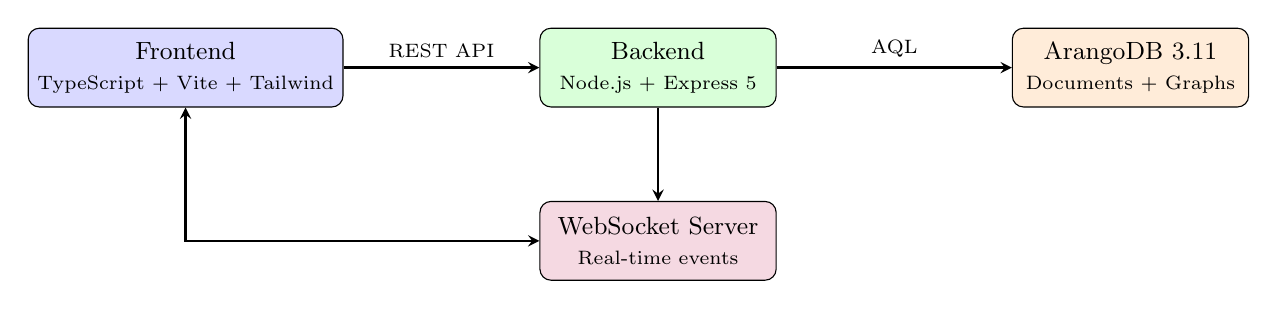
\begin{tikzpicture}[
      box/.style={draw, rounded corners, minimum width=3cm,
                  minimum height=1cm, align=center, font=\small},
      arr/.style={->, thick, >=stealth}
    ]
      % Frontend
      \node[box, fill=blue!15] (fe) at (0,0)
        {Frontend\\{\scriptsize TypeScript + Vite + Tailwind}};
      % Backend
      \node[box, fill=green!15] (be) at (6,0)
        {Backend\\{\scriptsize Node.js + Express 5}};
      % Database
      \node[box, fill=orange!15] (db) at (12,0)
        {ArangoDB 3.11\\{\scriptsize Documents + Graphs}};
      % WebSocket
      \node[box, fill=purple!15] (ws) at (6,-2.2)
        {WebSocket Server\\{\scriptsize Real-time events}};

      \draw[arr] (fe) -- node[above]{\scriptsize REST API} (be);
      \draw[arr] (be) -- node[above]{\scriptsize AQL} (db);
      \draw[arr, <->] (fe) |- (ws);
      \draw[arr] (be) -- (ws);
    \end{tikzpicture}
  \end{center}
  \vspace{0.5em}
  \begin{itemize}
    \item \textbf{Deployment:} Docker Compose (3 services: DB, backend, frontend)
    \item \textbf{Frontend:} Hyperscript DOM library + Tailwind CSS + Anime.js
    \item \textbf{Auth:} Client-side Argon2i (libsodium) $\rightarrow$ server SHA-256
  \end{itemize}
\note{
The architecture follows a clean three-tier pattern.
The frontend is a TypeScript single-page application built with Vite
and styled with Tailwind CSS. It communicates with the Express 5 backend
via REST and also maintains a persistent WebSocket connection for
real-time updates.
The backend talks to ArangoDB using AQL---ArangoDB's query language.
Everything deploys as a Docker Compose stack with three services.
Authentication uses a secure SRP-inspired protocol: passwords are hashed
client-side with Argon2i via libsodium, then the server applies
an additional SHA-256 layer.
}
\end{frame}

% ============================================================
\section{Database Design}
% ============================================================

% --------------------------------------------------
% SLIDE 6: Data Model
% --------------------------------------------------
\begin{frame}{Multi-Model Database Design}
  \begin{columns}[T]
    \begin{column}{0.48\textwidth}
      \textbf{Document Collections:}
      \begin{itemize}
        \item \texttt{users} --- credentials, salts, tokens
        \item \texttt{entities} --- posts, comments, map locations, trial entities
        \item \texttt{follows} --- user $\rightarrow$ entity subscriptions
        \item \texttt{notifications} --- per-user alerts
        \item \texttt{trials} --- court cases with status, judges, votes
      \end{itemize}
    \end{column}
    \begin{column}{0.48\textwidth}
      \textbf{Edge Collection:}
      \begin{itemize}
        \item \texttt{entity\_references} --- directed edges
              connecting entities that reference each other
      \end{itemize}
      \vspace{0.5em}
      \begin{block}{Why Multi-Model?}
        \begin{itemize}
          \item Document storage for flexible schema evolution
          \item Graph edges for relationship traversal
          \item Single AQL query language for both
          \item No cross-system synchronisation needed
        \end{itemize}
      \end{block}
    \end{column}
  \end{columns}
\note{
The database design is the heart of this project.
We have five document collections for structured data storage
and one edge collection for the knowledge graph.
The entities collection is polymorphic---it stores posts, comments,
map locations, and trial entities with a type discriminator.
The edge collection entity\_references stores directed links
between entities, enabling graph traversal queries.
The key advantage is that both document queries and graph traversals
use the same AQL language, eliminating the impedance mismatch
that would occur with separate database systems.
}
\end{frame}

% --------------------------------------------------
% SLIDE 7: Key AQL Queries
% --------------------------------------------------
\begin{frame}[fragile]{Representative AQL Queries}
  \textbf{1. Reference Discovery (Graph Traversal):}
  \begin{lstlisting}[language=SQL]
FOR v, e IN 1..1 OUTBOUND @entityId entity_references
  RETURN { entity: v, edge: e }
  \end{lstlisting}
  \vspace{0.3em}
  \textbf{2. Degree of Separation (Shortest Path):}
  \begin{lstlisting}[language=SQL]
FOR v IN OUTBOUND SHORTEST_PATH
  @fromId TO @toId entity_references
  RETURN v
  \end{lstlisting}
  \vspace{0.3em}
  \textbf{3. Full-Text Search:}
  \begin{lstlisting}[language=SQL]
FOR e IN entities
  FILTER CONTAINS(LOWER(e.title), LOWER(@query))
      OR CONTAINS(LOWER(e.body), LOWER(@query))
  RETURN e
  \end{lstlisting}
\note{
Here are three representative AQL queries that power the research features.
The first uses a graph traversal to find all entities referenced by a given entity.
The second uses ArangoDB's built-in SHORTEST\_PATH function to find the
minimum number of hops between any two entities---this is the
degree-of-separation feature.
The third performs full-text search across entity titles and bodies.
Notice how all three queries use the same AQL syntax,
whether they are document queries or graph traversals.
This uniformity is a major advantage of the multi-model approach.
}
\end{frame}

% ============================================================
\section{Feature Walkthrough}
% ============================================================

% --------------------------------------------------
% SLIDE 8: Landing Page
% --------------------------------------------------
\begin{frame}{Landing Page}
  \begin{center}
    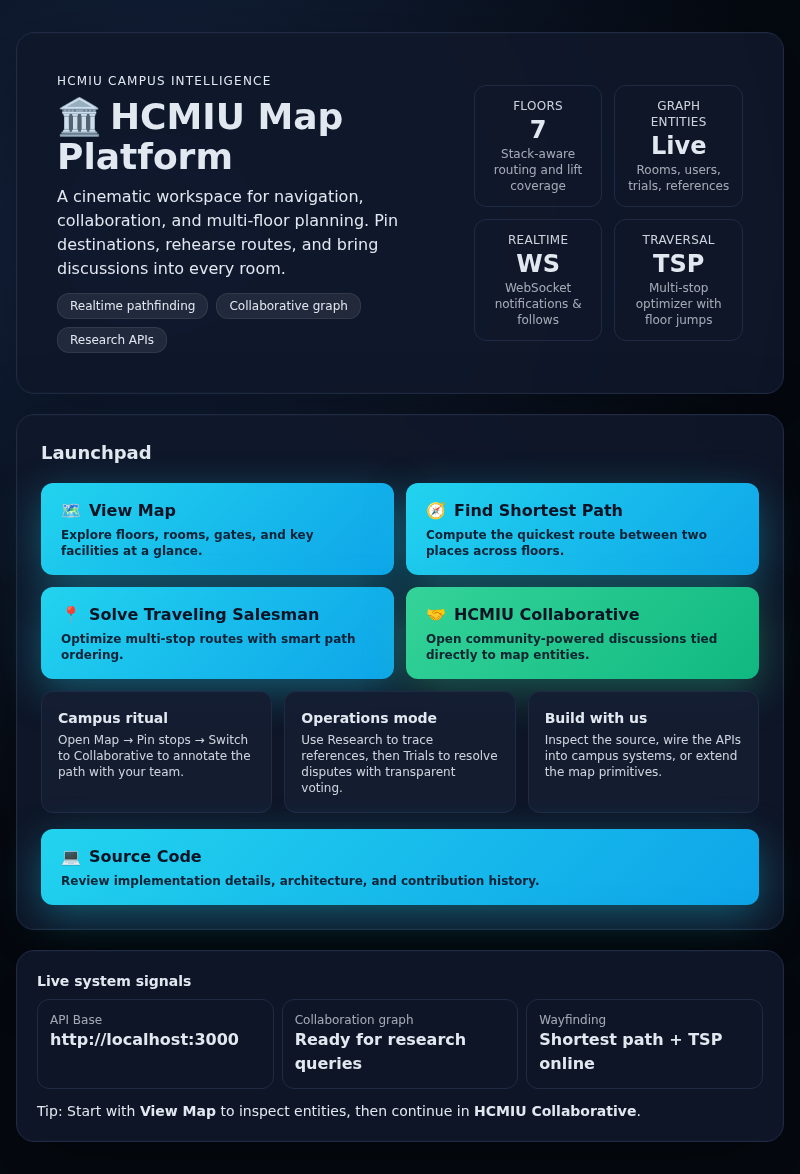
\includegraphics[width=0.72\textwidth]{landing-page.png}
  \end{center}
  \vspace{-0.3em}
  {\small Four main entry points: View Map, Shortest Path,
   Traveling Salesman, and HCMIU Collaborative.
   Live system signals show API status, graph readiness,
   and wayfinding availability.}
\note{
This is the landing page of the application.
It provides four main entry points corresponding to the major features:
View Map for floor exploration, Find Shortest Path for point-to-point
navigation, Solve Traveling Salesman for multi-stop optimization,
and HCMIU Collaborative for the knowledge graph platform.
At the bottom, live system signals display the health of the backend API,
the collaboration graph, and the wayfinding engine.
The design uses a dark theme with color-coded feature cards.
}
\end{frame}

% --------------------------------------------------
% SLIDE 9: Map View
% --------------------------------------------------
\begin{frame}{Interactive Campus Map}
  \begin{center}
    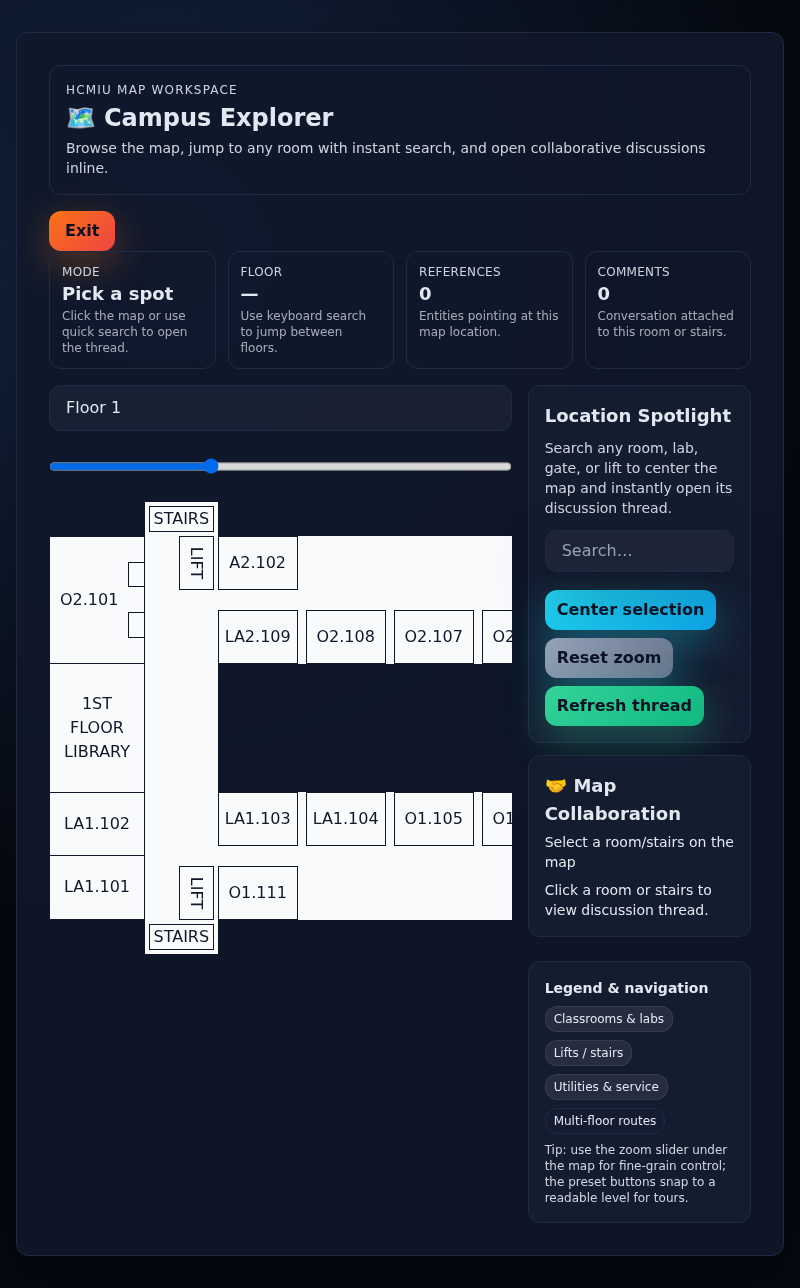
\includegraphics[width=0.72\textwidth]{map-view-page.png}
  \end{center}
  \vspace{-0.3em}
  {\small 7-floor interactive map with zoom/pan, room search,
   and direct links to collaborative discussions per location.}
\note{
The map view shows a detailed floor plan of the HCMIU campus.
On the left is the interactive SVG map with zoom and pan controls.
Users can switch between all seven floors using a dropdown.
On the right panel, there is a quick search box with autocomplete
for all named rooms. When a room is selected, the panel shows
its metadata including reference count and comment count,
plus a preview of the discussion thread attached to that location.
The ``Open in Collaborative'' link takes users directly to the
full discussion page for that room entity.
This bridges the gap between physical navigation and knowledge sharing.
}
\end{frame}

% --------------------------------------------------
% SLIDE 10: Pathfinding Algorithms
% --------------------------------------------------
\begin{frame}{Pathfinding Algorithms}
  \begin{columns}[T]
    \begin{column}{0.48\textwidth}
      \textbf{Shortest Path (BFS)}
      \begin{itemize}
        \item Breadth-first search on grid graph
        \item Handles \textbf{inter-floor routing} via stairs and lifts
        \item Visual path overlay on floor maps
        \item Time complexity: $O(V + E)$
      \end{itemize}
      \vspace{0.5em}
      \textbf{User Flow:}\\
      Select start $\rightarrow$ Select end $\rightarrow$\\
      View floor-by-floor directions
    \end{column}
    \begin{column}{0.48\textwidth}
      \textbf{Traveling Salesman (Held--Karp)}
      \begin{itemize}
        \item Bitmask dynamic programming
        \item Optimal visit order for $n$ destinations
        \item Multi-floor route planning
        \item Time complexity: $O(2^n \cdot n^2)$
      \end{itemize}
      \vspace{0.5em}
      \textbf{User Flow:}\\
      Add locations $\rightarrow$ Solve $\rightarrow$\\
      View optimised route with total distance
    \end{column}
  \end{columns}
\note{
The system implements two pathfinding algorithms.
The shortest path finder uses BFS on the campus grid graph.
It automatically handles inter-floor routing by detecting when a path
needs to go through stairs or lifts, then showing directions
floor by floor.
The Traveling Salesman solver uses the Held-Karp algorithm---a
bitmask dynamic programming approach with time complexity
O of 2-to-the-n times n-squared.
This finds the optimal visit order for multiple destinations.
Both algorithms visualise results as colored path overlays
on the floor maps, making it easy to follow directions physically.
}
\end{frame}

% --------------------------------------------------
% SLIDE 11: Collaborative Platform
% --------------------------------------------------
\begin{frame}{Collaborative Knowledge Graph}
  \begin{center}
    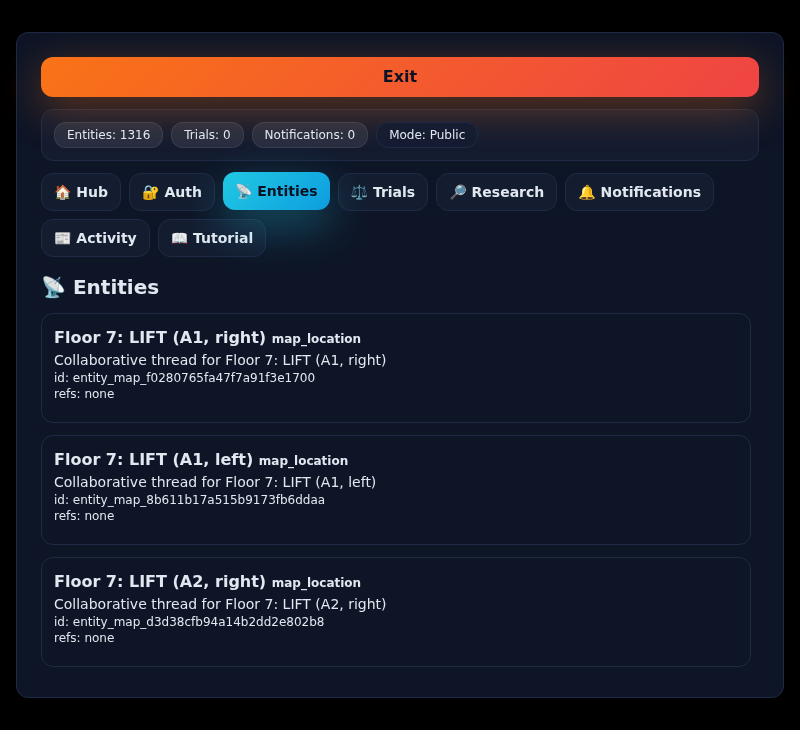
\includegraphics[width=0.68\textwidth]{collaborative-page.png}
  \end{center}
  \vspace{-0.3em}
  {\small Entity-based discussions, cross-references, follow/notification
   system, and real-time WebSocket updates.}
\note{
The collaborative page is the social backbone of the platform.
Every element in the system---rooms, users, posts, comments, trials---is
treated as a first-class entity in the knowledge graph.
Users can create discussion posts, attach comments to any entity,
and add cross-references to build a connected knowledge base.
The follow system lets users subscribe to entities and receive
notifications when new comments are added.
All changes propagate in real time via WebSockets---when one user
posts a comment, all connected clients see it instantly.
The navigation tabs at the top provide access to the Hub, Auth,
Entities, Trials, Research, Notifications, and Activity sections.
}
\end{frame}

% --------------------------------------------------
% SLIDE 12: Trial System
% --------------------------------------------------
\begin{frame}{Court of Justice --- Trial System}
  \begin{center}
    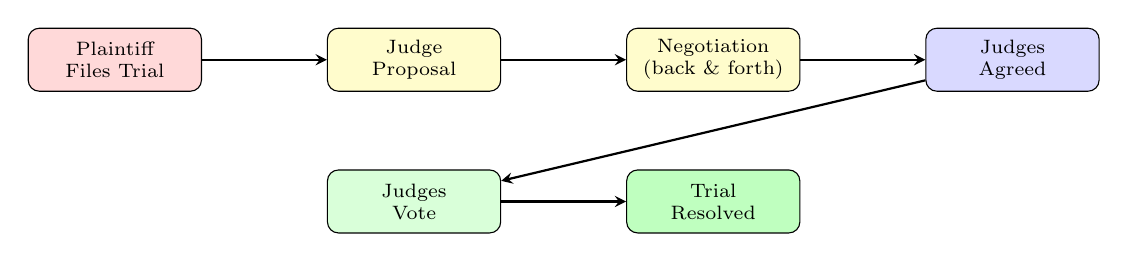
\begin{tikzpicture}[
      state/.style={draw, rounded corners, minimum width=2.2cm,
                    minimum height=0.8cm, align=center, font=\scriptsize},
      arr/.style={->, thick, >=stealth, font=\scriptsize}
    ]
      \node[state, fill=red!15] (file) at (0,0) {Plaintiff\\Files Trial};
      \node[state, fill=yellow!20] (prop) at (3.8,0) {Judge\\Proposal};
      \node[state, fill=yellow!20] (nego) at (7.6,0) {Negotiation\\(back \& forth)};
      \node[state, fill=blue!15] (agree) at (11.4,0) {Judges\\Agreed};
      \node[state, fill=green!15] (vote) at (3.8,-1.8) {Judges\\Vote};
      \node[state, fill=green!25] (resolve) at (7.6,-1.8) {Trial\\Resolved};

      \draw[arr] (file) -- (prop);
      \draw[arr] (prop) -- (nego);
      \draw[arr] (nego) -- (agree);
      \draw[arr] (agree) -- (vote);
      \draw[arr] (vote) -- (resolve);
    \end{tikzpicture}
  \end{center}
  \vspace{0.3em}
  \begin{itemize}
    \item Plaintiff files trial against defendant over a disputed entity
    \item Both parties negotiate judge selection (proposal $\leftrightarrow$ counter-proposal)
    \item Agreed judges cast votes: \texttt{plaintiff} / \texttt{defendant} / \texttt{no\_winner}
    \item Comments tagged by role: \texttt{[plaintiff]}, \texttt{[defendant]}, \texttt{[judge]}, \texttt{[spectator]}
  \end{itemize}
\note{
The Court of Justice is one of the most innovative features.
It provides a structured workflow for resolving disputes about
campus knowledge.
A plaintiff files a trial against a defendant, specifying the
entity under dispute. Then the two parties negotiate on who the
judges should be through a back-and-forth proposal mechanism.
Once both sides agree, the judges cast their votes.
Throughout the process, all participants can comment,
and their comments are tagged with their role.
This creates a transparent, auditable record of the dispute resolution.
The trial entity itself becomes part of the knowledge graph,
maintaining full traceability.
}
\end{frame}

% --------------------------------------------------
% SLIDE 13: Research Tools
% --------------------------------------------------
\begin{frame}{Research \& Knowledge Graph Tools}
  \begin{columns}[T]
    \begin{column}{0.48\textwidth}
      \textbf{Reference Discovery}
      \begin{itemize}
        \item Query entities by ID
        \item View all outbound references
        \item Explore the citation network
      \end{itemize}
      \vspace{0.5em}
      \textbf{Full-Text Search}
      \begin{itemize}
        \item Search across all entity titles and bodies
        \item Keyword-based discovery
        \item Cross-entity relationship finding
      \end{itemize}
    \end{column}
    \begin{column}{0.48\textwidth}
      \textbf{Degree of Separation}
      \begin{itemize}
        \item Find shortest reference path between any two entities
        \item Uses ArangoDB's native \texttt{SHORTEST\_PATH} function
        \item Visualises intermediate hops
      \end{itemize}
      \vspace{0.5em}
      \textbf{Mention Discovery}
      \begin{itemize}
        \item Find which entities mention a given entity
        \item Reverse reference traversal
        \item Map cross-entity relationships
      \end{itemize}
    \end{column}
  \end{columns}
\note{
The Research section provides four powerful tools that exploit
the graph model.
Reference Discovery lets users look up any entity and see all
the entities it references---essentially browsing the citation network.
Full-Text Search performs keyword searches across all entity titles
and bodies, useful for discovering related discussions.
Degree of Separation uses ArangoDB's native SHORTEST\_PATH function
to find the minimum number of reference hops between any two entities.
This is analogous to the ``six degrees of separation'' concept
but applied to campus knowledge.
Mention Discovery performs reverse traversal---finding which entities
reference a given entity, revealing unexpected connections.
}
\end{frame}

% ============================================================
\section{Real-Time \& WebSocket}
% ============================================================

% --------------------------------------------------
% SLIDE 14: Real-Time Architecture
% --------------------------------------------------
\begin{frame}{Real-Time Updates via WebSocket}
  \begin{columns}[T]
    \begin{column}{0.55\textwidth}
      \textbf{Event Types:}
      \begin{itemize}
        \item \texttt{entity.created} --- new post or comment
        \item \texttt{entity.updated} --- edit to existing entity
        \item \texttt{entity.deleted} --- entity removed
        \item \texttt{trial.created} --- new trial filed
        \item \texttt{trial.updated} --- vote or status change
        \item \texttt{notification.created} --- user alert
      \end{itemize}
    \end{column}
    \begin{column}{0.42\textwidth}
      \begin{block}{Design Decisions}
        \begin{itemize}
          \item RFC 6455 WebSocket protocol
          \item Token-authenticated connections
          \item Server-push model (no polling)
          \item All connected clients auto-refresh
        \end{itemize}
      \end{block}
    \end{column}
  \end{columns}
  \vspace{0.5em}
  \textbf{Result:} When User~A posts a comment, User~B sees it
  instantly without page refresh---verified in multi-user E2E tests.
\note{
Real-time updates are essential for a collaborative platform.
We use the WebSocket protocol---RFC 6455---with token-based authentication.
When a client connects, it provides its bearer token as a query parameter.
The server then pushes events to all relevant connected clients
whenever data changes occur.
There are six event types covering entity CRUD operations,
trial updates, and notifications.
This was verified through automated multi-user end-to-end tests
using Puppeteer, where two browser instances interact simultaneously
and changes appear instantly on both screens.
}
\end{frame}

% ============================================================
\section{Technology \& Testing}
% ============================================================

% --------------------------------------------------
% SLIDE 15: Technology Stack & Testing
% --------------------------------------------------
\begin{frame}{Technology Stack \& Testing}
  \begin{columns}[T]
    \begin{column}{0.48\textwidth}
      \textbf{Technology Stack:}
      \begin{center}
      \begin{tabular}{ll}
        \toprule
        \textbf{Layer} & \textbf{Technology} \\
        \midrule
        Frontend  & TypeScript, Vite, Tailwind \\
        UI        & Hyperscript, Anime.js \\
        Backend   & Node.js, Express 5 \\
        Database  & ArangoDB 3.11 \\
        Real-time & WebSocket (ws) \\
        Auth      & libsodium (Argon2i) \\
        Deploy    & Docker Compose \\
        \bottomrule
      \end{tabular}
      \end{center}
    \end{column}
    \begin{column}{0.48\textwidth}
      \textbf{Testing \& Validation:}
      \begin{itemize}
        \item \textbf{API unit tests} --- all REST endpoints
        \item \textbf{E2E tests} --- full Docker Compose stack
        \item \textbf{Backend stress benchmark visualisations} --- throughput and latency charts
        \item \textbf{8 demo videos} --- Puppeteer-automated screen recordings covering:
          \begin{itemize}
            \item Map navigation
            \item Multi-user real-time
            \item Trial system workflow
            \item Research tools (4 demos)
            \item General platform overview
          \end{itemize}
      \end{itemize}
    \end{column}
  \end{columns}
\note{
The technology stack was chosen for developer productivity
and architectural simplicity.
TypeScript provides type safety on the frontend.
Express 5 is the latest major version with improved async support.
ArangoDB 3.11 gives us native multi-model capabilities.
WebSocket via the ws library provides efficient real-time communication.
For testing, we have API unit tests for all REST endpoints,
full end-to-end tests using Docker Compose,
and eight automated demo videos generated with Puppeteer
that exercise every major workflow.
These demos serve as both regression tests and documentation---they
show exactly how each feature works through real browser interactions.
We also visualise backend stress benchmark performance on the next
two slides using throughput and latency percentile charts.
}
\end{frame}

% --------------------------------------------------
% SLIDE 16: Benchmark Throughput
% --------------------------------------------------
\begin{frame}{Benchmarking: Throughput by Scenario}
  \begin{center}
    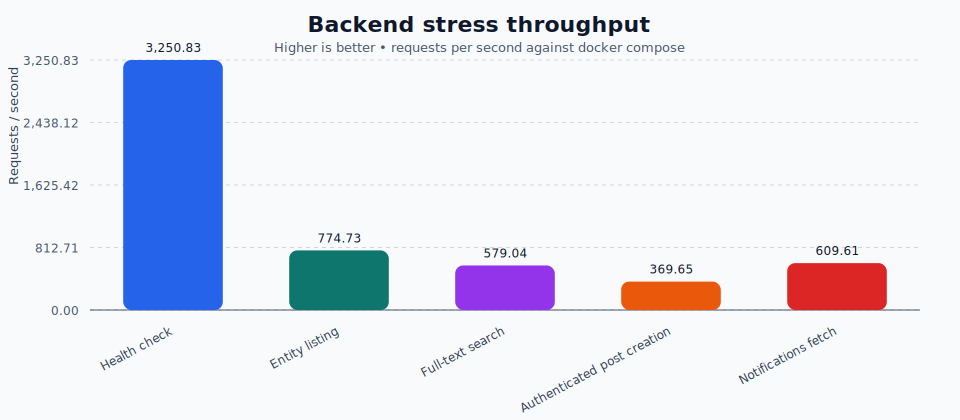
\includegraphics[width=\textwidth,height=0.82\textheight,keepaspectratio]{../docs/benchmarks/backend-stress-throughput.png}
  \end{center}
\note{
This chart summarizes throughput across benchmark scenarios.
It highlights that simple endpoints like health checks achieve the highest
request rates, while heavier features such as full-text and mention queries
remain stable at lower but consistent throughput.
}
\end{frame}

% --------------------------------------------------
% SLIDE 17: Benchmark Latency
% --------------------------------------------------
\begin{frame}{Benchmarking: Latency Percentiles by Scenario}
  \begin{center}
    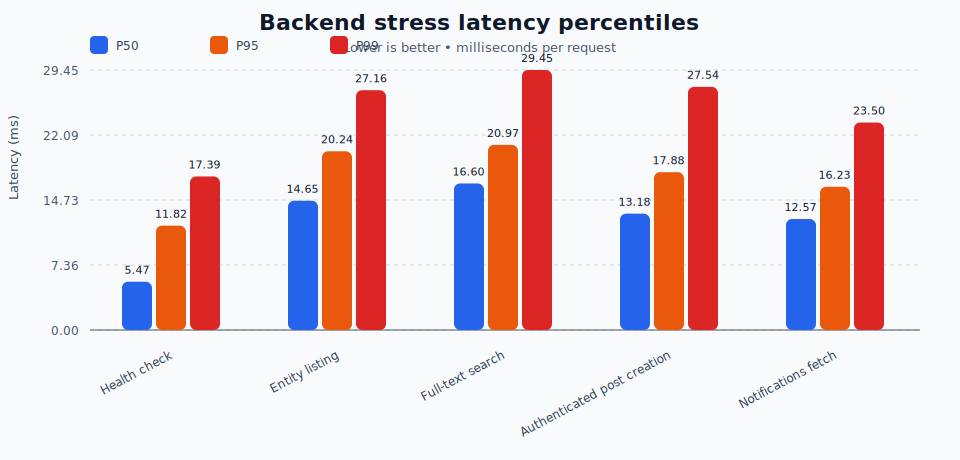
\includegraphics[width=\textwidth,height=0.82\textheight,keepaspectratio]{../docs/benchmarks/backend-stress-latency.png}
  \end{center}
\note{
This latency chart compares p50, p95, and p99 by scenario.
Most scenarios stay in a low-latency band, and the percentile spread helps
us reason about tail behavior under load rather than relying on single
headline numbers.
}
\end{frame}

% ============================================================
\section{Conclusion}
% ============================================================

% --------------------------------------------------
% SLIDE 18: Conclusions & Future Work
% --------------------------------------------------
\begin{frame}{Conclusions \& Future Work}
  \textbf{Key Contributions:}
  \begin{enumerate}
    \item Demonstrated that a \textbf{multi-model DBMS} (ArangoDB) can effectively
          serve both document storage and graph traversal needs in a single engine
    \item Built a \textbf{complete campus platform} combining wayfinding,
          collaboration, governance, and research
    \item Implemented \textbf{graph-native features} (reference discovery,
          degree-of-separation, mention traversal) that would be complex
          in a document-only or relational system
    \item Validated correctness through \textbf{comprehensive automated testing}
  \end{enumerate}
  \vspace{0.5em}
  \textbf{Limitations \& Future Work:}
  \begin{itemize}
    \item Access control is creator-based; role-based permissions needed
    \item Event ordering relies on eventual consistency; formal guarantees desirable
    \item Map data is hardcoded; a map editor would improve extensibility
    \item Extend benchmarking to sustained mixed-write workloads and larger datasets
  \end{itemize}
\note{
To summarise, this project makes four key contributions.
First, it demonstrates that ArangoDB's multi-model architecture
can handle both document storage and graph queries effectively,
reducing the need for polyglot persistence.
Second, it delivers a complete campus platform that goes beyond
simple maps to include collaboration, governance, and research.
Third, graph-native features like degree-of-separation queries
showcase capabilities that would be complex in traditional databases.
Fourth, comprehensive testing---including 8 automated demo videos---ensures
correctness and serves as living documentation.
For future work, we identified four areas: role-based access control,
formal consistency guarantees, a dynamic map editor,
and broader benchmarking under sustained mixed workloads.
}
\end{frame}

% --------------------------------------------------
% SLIDE 19: References
% --------------------------------------------------
\begin{frame}{References}
  \begin{thebibliography}{9}
    \bibitem{stonebraker2005onesize}
    M.~Stonebraker and U.~\c{C}etintemel,
    ``One Size Fits All: An Idea Whose Time Has Come and Gone,''
    \emph{Proc.\ ICDE}, pp.~2--11, 2005.

    \bibitem{sadalage2012nosql}
    P.~Sadalage and M.~Fowler,
    \emph{NoSQL Distilled: A Brief Guide to the Emerging World of
    Polyglot Persistence},
    Addison-Wesley, 2012.

    \bibitem{arangodb_multimodel}
    ArangoDB Inc.,
    ``ArangoDB---the Multi-Model NoSQL Database,''
    \url{https://www.arangodb.com/}, 2024.

    \bibitem{zimmerman2006wayfinding}
    A.~Zimmerman and M.~Martin,
    ``Post-occupancy evaluation: benefits and barriers,''
    \emph{Building Research \& Information},
    vol.~29, no.~2, pp.~168--174, 2001.
  \end{thebibliography}
\note{
These are the main references that informed the design decisions.
Stonebraker's seminal work on the limitations of one-size-fits-all
databases motivated our choice of a multi-model approach.
Sadalage and Fowler's book on NoSQL provided context on
polyglot persistence trade-offs.
The ArangoDB documentation was the primary technical reference.
And Zimmerman's work on wayfinding informed the navigation design.
Thank you for your attention. I am happy to take questions.
}
\end{frame}

% --------------------------------------------------
% SLIDE 20: Thank You / Q&A
% --------------------------------------------------
\begin{frame}
  \begin{center}
    \vfill
    {\Huge Thank You}\\[1em]
    {\Large Questions?}\\[1.5em]
    {\normalsize
      \textbf{Live Demo:} \url{https://hcmiumap.huynhtrankhanh.com/}\\[0.3em]
      \textbf{Source Code:} \url{https://github.com/huynhtrankhanh/hcmiu-map-collaborative}
    }
    \vfill
  \end{center}
\note{
Thank you for listening. The live demo is available at the URL shown.
The full source code, including all automated tests and demo video
generation scripts, is open-source on GitHub.
I am happy to answer any questions about the architecture,
database design, algorithms, or implementation details.
}
\end{frame}

\end{document}
